\label{experiments}
In this chapter we present in the first part the problems on which the NRAM is trained, finishing by comparing the results and by presenting the circuits learned by the neural networks.

\section{Tasks}
The following are the description of the executed task used in our experiments. In the description, big and small letters represents respectively arrays and pointers, \textit{NULL} denotes the value 0 and is used as an ending character or in the lists, as a placeholder for missing next element. In the experiments, along the initial and desired memories, are also generated the cost masks that used during the cost calculation as attention mechanisms.

\subsection{Access}
Given a value $k$ and an array \textbf{A}, return $\textbf{A}[k]$. Input is given as $k,\ A[0],\ \dots,\ $\\$\textbf{A}[n-1],\ \textit{NULL}$ and the network should replace the first memory cell with $\textbf{A}[k]$. An example is visible in Figure \ref{fig:access-example}.
\begin{table}[h!]
	\centering
	\begin{tabular}{|c|c|c|c|c|c|c|c|c|c|}
		\hline
		\multicolumn{10}{|c|}{\textbf{Initial memory}} \\ \hline
		\textbf{4} & 5 & 1 & 4 & \underline{7} & 2 & 8 & 3 & 6 & 0 \\ \hline\hline\hline
		\multicolumn{10}{|c|}{\textbf{Desired memory}} \\ \hline
		\textbf{7} & 5 & 1 & 4 & 7 & 2 & 8 & 3 & 6 & 0 \\ \hline\hline\hline
		\multicolumn{10}{|c|}{\textbf{Cost mask}} \\ \hline
		1 & 1 & 1 & 1 & 1 & 1 & 1 & 1 & 1 & 1 \\ \hline
	\end{tabular}
	\caption{Expected behaviour with the task Access - the first value is the pointer in the sequence A to which the NRAM should access.}
	\label{fig:access-example}
\end{table}
\FloatBarrier
\subsection{Increment}
Given an array $\textbf{A}$, increment all its elements by 1. Input is given as $\textbf{A}[0],\ \dots,\ \textbf{A}[n-1],\ \textit{NULL}$ and the expected output is $\textbf{A}[0] + 1,\ \dots,\ A[n-1] + 1$. An example is visible in Figure \ref{fig:increment-example}.
\begin{table}[h!]
	\centering
	\begin{tabular}{|c|c|c|c|c|c|c|c|c|c|}
		\hline
		\multicolumn{10}{|c|}{\textbf{Initial memory}} \\ \hline
		5 & 5 & 9 & 4 & 7 & 8 & 0 & 0 & 0 & 0 \\ \hline\hline\hline
		\multicolumn{10}{|c|}{\textbf{Desired memory}} \\ \hline
		6 & 6 & 0 & 4 & 8 & 9 & 0 & 0 & 0 & 0 \\ \hline\hline\hline
		\multicolumn{10}{|c|}{\textbf{Cost mask}} \\ \hline
		1 & 1 & 1 & 1 & 1 & 1 & 1 & 1 & 1 & 1 \\ \hline
	\end{tabular}
	\caption{Expected behaviour with the task Increment - each element must be incremented by one, also considering the interval of the values N.}
	\label{fig:increment-example}
\end{table}
\FloatBarrier
\subsection{Copy}
Given an array and a pointer to the destination, copy all elements from the array to the given location. Input is given as $p,\ \textbf{A}[0],\ \dots,\ \textbf{A}[n-1]$ where $p$ points to one element after $\textbf{A}[n-1]$. The expected output is $\textbf{A}[0],\ \dots,\ \textbf{A}[n-1]$ at positions $p,\ \dots,\ p+n-1$ respectively. An example is visible in Figure \ref{fig:copy-example}.
\begin{table}[h!]
	\centering
	\begin{tabular}{|c|c|c|c|c|c|c|c|c|c|}
		\hline
		\multicolumn{10}{|c|}{\textbf{Initial memory}} \\ \hline
		\textbf{5} & 5 & 1 & 4 & 7 & \underline{0} & 0 & 0 & 0 & 0 \\ \hline\hline\hline
		\multicolumn{10}{|c|}{\textbf{Desired memory}} \\ \hline
		\textbf{5} & 5 & 1 & 4 & 7 & 5 & 1 & 4 & 7 & 0 \\ \hline\hline\hline
		\multicolumn{10}{|c|}{\textbf{Cost mask}} \\ \hline
		0 & 0 & 0 & 0 & 0 & 1 & 1 & 1 & 1 & 1 \\ \hline
	\end{tabular}
	\caption{Expected behaviour with the task Copy -the first value is the pointer to the memory to which the NRAM should starts copy the sequence A. }
	\label{fig:copy-example}
\end{table}
\FloatBarrier
\subsection{Reverse}
Given an array and a pointer to the destination, copy all elements from the array in reversed order. Input is given as $p,\ \textbf{A}[0],\ \dots,\ \textbf{A}[n-1]$ where $p$ points one element after $\textbf{A}[n-1]$. The expected output is $\textbf{A}[n-1],\ \dots,\ \textbf{A}[0]$ at positions $p,\ \dots,\ p+n-1$ respectively. An example is visible in Figure \ref{fig:reverse-example}.
\begin{table}[h!]
	\centering
	\begin{tabular}{|c|c|c|c|c|c|c|c|c|c|}
		\hline
		\multicolumn{10}{|c|}{\textbf{Initial memory}} \\ \hline
		\textbf{5} & 5 & 1 & 4 & 7 & \underline{0} & 0 & 0 & 0 & 0 \\ \hline\hline\hline
		\multicolumn{10}{|c|}{\textbf{Desired memory}} \\ \hline
		\textbf{5} & 5 & 1 & 4 & 7 & 7 & 4 & 1 & 5 & 0 \\ \hline\hline\hline
		\multicolumn{10}{|c|}{\textbf{Cost mask}} \\ \hline
		0 & 0 & 0 & 0 & 0 & 1 & 1 & 1 & 1 & 1 \\ \hline
	\end{tabular}
	\caption{Expected behaviour with the task Reverse - the first value is the pointer to the memory to which the NRAM should starts reverse the sequence A.}
	\label{fig:reverse-example}
\end{table}
\FloatBarrier
\subsection{Swap}
Given two pointers $p,\ q$ and an array \textbf{A}, swap elements $\textbf{A}[p]$ and $\textbf{A}[q]$. Input is given as $p,\ q,\ \textbf{A}[0],\ \dots,\ \textbf{A}[p],\ \dots,\ \textbf{A}[q],\ \dots,\ \textbf{A}[n-1],\ 0$. The expected modified array \textbf{A} is: $\textbf{A}[0],\ \dots,\ \textbf{A}[q],\ \dots,\ \textbf{A}[p],\ \dots,\ \textbf{A}[n-1]$. An example is visible in Figure \ref{fig:swap-example}.
\begin{table}[h!]
	\centering
	\begin{tabular}{|c|c|c|c|c|c|c|c|c|c|}
		\hline
		\multicolumn{10}{|c|}{\textbf{Initial memory}} \\ \hline
		\textbf{5} & \textbf{7} & 1 & 4 & 7 & \underline{3} & 6 & \underline{8} & 1 & 0 \\ \hline\hline\hline
		\multicolumn{10}{|c|}{\textbf{Desired memory}} \\ \hline
		\textbf{5} & \textbf{7} & 1 & 4 & 7 & \underline{8} & 6 & \underline{3} & 1 & 0 \\ \hline\hline\hline
		\multicolumn{10}{|c|}{\textbf{Cost mask}} \\ \hline
		0 & 0 & 1 & 1 & 1 & 1 & 1 & 1 & 1 & 1 \\ \hline
	\end{tabular}
	\caption{Expected behaviour with the task Swap - the first two value is the pointer in the sequence A that should be swapped.}
	\label{fig:swap-example}
\end{table}
\FloatBarrier

\subsection{Permutation}
Given two arrays of n elements: P (contains a permutation of numbers $0,\ \dots,\ n-1$) and \textbf{A} (contains random elements), permutate \textbf{A} according to P. Input is given as a, $P[0],\ \dots,\ P[n-1],\ \textbf{A}[0],\ ...,\ \textbf{A}[n-1]$, where a is a pointer to the array \textbf{A}. The expected output is $\textbf{A}[P[0]],\ \dots,\ \textbf{A}[P[n-1]]$, which should override the array P. An example is visible in Figure \ref{fig:permutation-example}.
\begin{table}[h!]
	\centering
	\begin{tabular}{|c|c|c|c|c|c|c|c|c|c|}
		\hline
		\multicolumn{10}{|c|}{\textbf{Initial memory}} \\ \hline
		\textbf{5} & 2 & 1 & 0 & 3 & \underline{3} & 6 & 8 & 1 & 0 \\ \hline\hline\hline
		\multicolumn{10}{|c|}{\textbf{Desired memory}} \\ \hline
		\textbf{5} & 8 & 6 & 2 & 1 & \underline{3} & 6 & 8 & 1 & 0 \\ \hline\hline\hline
		\multicolumn{10}{|c|}{\textbf{Cost mask}} \\ \hline
		0 & 1 & 1 & 1 & 1 & 0 & 0 & 0 & 0 & 0 \\ \hline
	\end{tabular}
	\caption{Expected behaviour with the task Swap - the first two value is the pointer in the sequence A that should be swapped.}
	\label{fig:permutation-example}
\end{table}
\FloatBarrier

\subsection{Sum}
Given pointers to 2 arrays \textbf{A} and \textbf{B}, and the pointer to the output $o$, sum the two arrays into one array. The input is given as: $a,\ b,\ o,\ \textbf{A}[0],\ \dots,\ \textbf{A}[n-1],\ G,\ \textbf{B}[0],\ \dots,\ \textbf{B}[m-1],\ G$, where $a$ points to first element of \textbf{A}, $b$ points to the first element of \textbf{B}, $o$ points to first element of output array and $G$ is a special guardian value. The $\textbf{A}+\textbf{B}$ array should be written starting from position $o$. An example is visible in Figure \ref{fig:sum-example}.
\begin{table}[h!]
	\centering
	\begin{tabular}{|c|c|c|c|c|c|c|c|c|c|c|c|}
		\hline
		\multicolumn{12}{|c|}{\textbf{Initial memory}} \\ \hline
		\textbf{3} & \textbf{6} & \textbf{9} & \underline{3} & 5 & 0 & \underline{4} & 6 & 0 & \underline{0} & 0 & 0 \\ \hline\hline\hline
		\multicolumn{12}{|c|}{\textbf{Desired memory}} \\ \hline
		\textbf{3} & \textbf{6} & \textbf{9} & \underline{3} & 5 & 0 & \underline{4} & 6 & 0 & \underline{7} & 11 & 0 \\ \hline\hline\hline
		\multicolumn{12}{|c|}{\textbf{Cost mask}} \\ \hline
		0 & 0 & 0 & 0 & 0 & 0 & 0 & 0 & 0 & 1 & 1 & 0 \\ \hline
	\end{tabular}
	\caption{Expected behaviour with the task Sum - the values of the two arrays are summed up and copied starting from the index $o$.}
	\label{fig:sum-example}
\end{table}
\FloatBarrier

\section{The generalization problem}
Generalization means the capacity of a neural network to recognize patterns never seen before in new examples. In a classic classification problem this means that the neural network should recognize the patterns in the features presented to it, classifying them with the correct label. The same concept can be also applied to NRAM, with some differences. Remembering that the training is made over memory with limited size and timesteps, with ``generalization capacity'' means that the controller should learns to create the right circuit also for examples\footnote{Please refer to Section \ref{subsubsec:nram-dataset} to see how the examples are formed.} with memory of different sizes and timesteps. As stated previously in the Paragraph \ref{subpar:curriculum-learning}, the Curriculum Learning is used to boost the training making the neural network more robust - in fact, the training over a specific memory size and timesteps could leads the objective function to have a value equal to zero, but this does not means that the neural network has learnt to generalize.

\section{Results}
In the experiments we have follow what is do in the paper \cite{NRAM:2016}, training of NRAM with DENN and Theano on ``easy'' and ``hard'' tasks. The objectives are to compare the performances of DENN and Theano without Curriculum Learning and the performances between DENN and DENN with Curriculum Learning, focusing specially to the generalization capacity of the discovered solutions.\newline
\begin{table}[t]
	\centering

	\rowcolors{2}{white}{LightGray}
	\resizebox{\textwidth}{!}{\begin{tabular}{ccccccccc}
		\rowcolor{Gray} \textbf{Task} & \multicolumn{2}{c}{\textbf{Train complexity}} & \multicolumn{2}{c}{\textbf{Reached cost 0}} & \multicolumn{2}{c}{\textbf{Train error}} & \multicolumn{2}{c}{\textbf{Generalization}} \\
		\rowcolor{Gray} & No CL & CL & No CL & CL & No CL & CL & No CL & CL \\ \hline
		
		Access & \begin{tabular}{@{}c@{}c}
			$\textrm{len}(A) = 6$\\
			$t = 3$
		\end{tabular} & $\textrm{len}(A) \leq 10$ & \checkmark & \checkmark & 0 & 0 & \begin{tabular}{@{}c@{}c}Semi\\-perfect\end{tabular} & Perfect \\ 
		Increment & \begin{tabular}{@{}c@{}c}
			$\textrm{len}(A) = 9$\\
			$t = 9$
		\end{tabular} & $\textrm{len}(A) \leq 11$  & \checkmark & \checkmark & 0 & 0 & Perfect & Perfect \\
		Copy & \begin{tabular}{@{}c@{}c}
			$\textrm{len}(A) = 5$\\
			$t = 12$
		\end{tabular} & $\textrm{len}(A) \leq 9$  & \checkmark & $\times$ & 0 & --- & \begin{tabular}{@{}c@{}c}Semi\\-perfect\end{tabular} & --- \\ 
		Reverse & \begin{tabular}{@{}c@{}c}
			$\textrm{len}(A) = 4$\\
			$t = 9$
		\end{tabular} & $\textrm{len}(A) \leq 8$ & \checkmark & \checkmark & 0 & 0 & Perfect & Perfect \\ 
		Swap & \begin{tabular}{@{}c@{}c}
			$\textrm{len}(A) = 7$\\
			$t = 6$
		\end{tabular} & $\textrm{len}(A) \leq 7$ & \checkmark & $\times$ & 0 & --- & \begin{tabular}{@{}c@{}c}Semi\\-perfect\end{tabular} & --- \\ \hline\hline
		Permutation & $\textrm{len}(A) = 5$ & $\textrm{len}(A) \leq 20$ & $\times$ & $\times$ & --- & --- & --- & --- \\ 
		ListK & $\textrm{len}(list) = \_$ & $\textrm{len}(list) \leq \_$ & $\times$ & $\times$ & --- & --- & --- & ---\\ 
		ListSearch & $\textrm{len}(list) = \_$ & $\textrm{len}(list) \leq \_$ & $\times$ & $\times$ & --- & --- & --- & ---  \\ 
		Merge & \begin{tabular}{@{}c@{}c}$\textrm{len}(A)+\textrm{len}(B)$\\$= \_$\end{tabular} & \begin{tabular}{@{}c@{}c}$\textrm{len}(A)+\textrm{len}(B)$\\$\leq \_$\end{tabular} & $\times$ & $\times$ & --- & --- & --- & --- \\ 
		WalkBST & $\textrm{size}(tree) = \_$ & $\textrm{size}(tree) \leq \_$ & $\times$ & $\times$ & --- & --- & --- & --- \\ 
		Sum & \begin{tabular}{@{}c@{}c}$\textrm{len}(A)+\textrm{len}(B)$\\$= 6$\end{tabular}& \begin{tabular}{@{}c@{}c}$\textrm{len}(A)+\textrm{len}(B)$\\$ \leq 10$\end{tabular} & $\times$ & $\times$ & --- & --- & --- & --- \\
	\end{tabular}\label{tbl:denn-tests-results}}
	\caption{Results of the tests with DENN. The train complexity represents the maximum length of integers sequence A used in the training. The train error represents the lowest error rate reached by the trained neural networks. The generalization represents the behaviour of the neural networks with memory sequences longer and more timesteps with respect to those used in training. The evaluation is executed as in \cite{NRAM:2016}, except for the keyword \textbf{Semi-Perfect} which means that the found solution generalize well only with input sequences and timesteps compatible to those used in the training. With \textbf{---} we indicate the lack of informations due to non-convergence of controller.}
	
\end{table}

\begin{table}[t]
	\centering
	
	\rowcolors{2}{white}{LightGray}
	\resizebox{\textwidth}{!}{\begin{tabular}{ccccc}
		\rowcolor{Gray} \textbf{Task} & \textbf{Train complexity} & \textbf{Reached cost 0} & \textbf{Train error} & \textbf{Generalization} \\ \hline
		Access & \begin{tabular}{@{}c@{}c}
			$\textrm{len}(A) = 9$\\
			$t = 3$
		\end{tabular} & $\times$ & --- & --- \\ 
		Increment & \begin{tabular}{@{}c@{}c}
			$\textrm{len}(A) = 9$\\
			$t = 3$
		\end{tabular} & $\times$ & --- & --- \\
		Copy & \begin{tabular}{@{}c@{}c}
			$\textrm{len}(A) = 5$\\
			$t = 3$
		\end{tabular} & $\times$ & --- & ---  \\ 
		Reverse & \begin{tabular}{@{}c@{}c}
			$\textrm{len}(A) = 4$\\
			$t = 3$
		\end{tabular} & $\times$ & --- & --- \\ 
		Swap & \begin{tabular}{@{}c@{}c}
			$\textrm{len}(A) = 7$\\
			$t = 3$
		\end{tabular} & $\times$ & 
		--- & --- \\ \hline\hline
		Permutation & \begin{tabular}{@{}c@{}c}
			$\textrm{len}(A) = \_$\\
			$t = \_$
		\end{tabular} & $\times$ & --- & --- \\ 
		ListK & \begin{tabular}{@{}c@{}c}
			$\textrm{len}(list) = \_$\\
			$t = \_$
		\end{tabular} & $\times$ & --- & --- \\ 
		ListSearch & \begin{tabular}{@{}c@{}c}
			$\textrm{len}(list) = \_$\\
			$t = \_$
		\end{tabular} & $\times$ & --- & ---  \\ 
		Merge & \begin{tabular}{@{}c@{}c}$\textrm{len}(A)+\textrm{len}(B)$\\$= \_$\\$t=\_$\end{tabular} & $\times$ & --- & --- \\ 
		WalkBST & \begin{tabular}{@{}c@{}c}$\textrm{size}(tree) = \_$\\$t=\_$\end{tabular} & $\times$ & --- & ---  \\ 
		Sum & \begin{tabular}{@{}c@{}c}$\textrm{len}(A)+\textrm{len}(B)$\\$= \_$\\$t=\_$\end{tabular} & $\times$ & --- & --- \\
	\end{tabular}\label{tbl:adam-tests}}
	\caption{Results of the tests of Adam. The contained informations follows those in Table \ref{tbl:denn-tests-results}.}
\end{table}
The used variants of DE are \textbf{JADE}, \textbf{SHADE} and \textbf{L-SHADE}, which are combined with the mutation methods \textbf{DEGL} and \textbf{Current to p best} and the crossover method \textbf{bin}. We used in each tests a population of 100 individuals. For DEGL we used a neighborhood in the interval $[4, 8]$ and for Current to p best a $p = 0.1$. All the tests are executed with a feedforward neural network with two hidden levels, each containing 260 neurons. The training set is composed of batches of 1000 examples generated at runtime. The cost calculation has been done with the cost function showed in the Section \ref{subsec:cost-function}. The train error is calculated with the expression introduced in Paragraph \ref{subpar:curriculum-learning}. The generalization tests are executed with input sequences up to 1000 values. The Curriculum Learning was set up with an interval of batches between $[25, 250]$ and a threshold equal to 0.1. \newline\newline

\begin{table}[t]
	\centering
	\rowcolors{2}{LightGray}{white}
	\resizebox{\textwidth}{!}{\begin{tabular}{|c|cccccccccccc|cccccc|cc|}
		\hline
		\rowcolor{Gray}\textbf{Step} & 0 & 1 & 2 & 3 & 4 & 5 & 6 & 7 & 8 & 9 & 10 & 11 & \textit{r}0 & \textit{r}1 & \textit{r}2 & \textit{r}3 & \textit{r}4 & \textit{r}5 & Read & Write \\ \hline 
1 & 6 & 3 & 1 & 2 & 10 & 11 & 0 & 0 & 0 & 0 & 0 & 0 & 1 & 1 & 0 & 0 & 0 & 1 & p:0 & p:6 v:6 \\ 
2 & 6 & 3 & 1 & 2 & 10 & 11 & 6 & 0 & 0 & 0 & 0 & 0 & 2 & 2 & 0 & 0 & 0 & 2 & p:1 & p:10 v:3 \\ 
3 & 6 & 3 & 1 & 2 & 10 & 11 & 6 & 0 & 0 & 0 & 3 & 0 & 3 & 3 & 0 & 0 & 0 & 3 & p:2 & p:9 v:1 \\ 
4 & 6 & 3 & 1 & 2 & 10 & 11 & 6 & 0 & 0 & 1 & 3 & 0 & 4 & 4 & 0 & 0 & 0 & 4 & p:3 & p:8 v:2 \\ 
5 & 6 & 3 & 1 & 2 & 10 & 11 & 6 & 0 & 2 & 1 & 3 & 0 & 5 & 5 & 0 & 0 & 0 & 5 & p:4 & p:7 v:10 \\ 
6 & 6 & 3 & 1 & 2 & 10 & 11 & 6 & 10 & 2 & 1 & 3 & 0 & 6 & 6 & 0 & 0 & 0 & 6 & p:5 & p:6 v:11 \\ 
7 & 6 & 3 & 1 & 2 & 10 & 11 & 11 & 10 & 2 & 1 & 3 & 0 & 7 & 7 & 0 & 0 & 0 & 7 & p:6 & p:5 v:11 \\ 
8 & 6 & 3 & 1 & 2 & 10 & 11 & 11 & 10 & 2 & 1 & 3 & 0 & 8 & 8 & 0 & 0 & 0 & 8 & p:7 & p:4 v:10 \\ 
9 & 6 & 3 & 1 & 2 & 10 & 11 & 11 & 10 & 2 & 1 & 3 & 0 & 9 & 9 & 0 & 0 & 0 & 9 & p:8 & p:3 v:2 \\ 
10 & 6 & 3 & 1 & 2 & 10 & 11 & 11 & 10 & 2 & 1 & 3 & 0 & 10 & 10 & 0 & 0 & 0 & 10 & p:9 & p:2 v:1 \\ 
11 & 6 & 3 & 1 & 2 & 10 & 11 & 11 & 10 & 2 & 1 & 3 & 0 & 11 & 11 & 0 & 0 & 0 & 11 & p:10 & p:1 v:3\\ \hline 
\rowcolor{Gray}Final & 6 & 3 & 1 & 2 & 10 & 11 & 11 & 10 & 2 & 1 & 3 & 0 & 11 & 11 & 0 & 0 & 0 & 11 & $\times$ & $\times$ \\ \hline
	\end{tabular}}
	\label{tbl:example-memories-execution}
	\caption{Example of execution showing the memory, register and Read/Write gates states of Task Reverse with the controller discovered without the using of Curriculum Learning. The keywords \textbf{p} and \textbf{v} indicates respectively the pointer which is accessed and the value which is written. }
\end{table}
\iffalse
\begin{figure}[t]
	\centering
	\begin{tikzpicture}[samples=100,smooth, scale=.875]
			\begin{axis}[
 				axis x line=center,
  				axis y line=center,
 				xlabel={Sequence A length},
  				ylabel={Error rate},
    				x label style={at={(axis description cs:0.5,-0.115)},anchor=north},
    				y label style={at={(axis description cs:-0.115,.5)},rotate=90,anchor=south},    				
			    grid=both,
			    grid style={line width=.1pt, draw=gray!10},
			    major grid style={line width=.2pt,draw=gray!50},
			    xtick={10, 20, 30 50, 100, 500, 1000},
			    xmin=0, xmax=1000,
			    ymin=0, ymax=1,
				legend style={at={(0.5,-0.25)},anchor=north}		
			]
  				\addplot table{data/swap-error-rate-CL.txt};
  				\addlegendentry{Swap CL}
			\end{axis}
	\end{tikzpicture}
	\label{fig:nram-tests-error-rate-plot}
	\caption{Error rate of best controllers in generalization tests.}
\end{figure}
\fi
The training was executed using configurations of max int, timesteps and registers compatible with those used by Kurach et al. As showed in the Table \ref{tbl:denn-tests-results}, for the easy tasks trained with Differential Evolution without the Curriculum Learning we found a set of hyperparameter which reached error 0 during the training, even using shorter input sequences compared to those used in the paper. Differently from which declared in Kurach at al., for tasks Copy and Swap the search of hyperparameters has been difficulty. The same results was not reached in the training with Theano, as showed in \ref{tbl:adam-tests}. 
\begin{table}[h]
	\centering
	\rowcolors{2}{LightGray}{white}
	\begin{tabular}{c|ccccccccccccccc|cc}
		\rowcolor{Gray}\textbf{Step} & 0 & 1 & 2 & 3 & 4 & 5 & 6 & 7 & 8 & 9 & 10 & 11 & 12 & 13 & 14 & \textit{r}0 & \textit{r}1 \\ \hline 
1 & 4 & 7 & 8 & 3 & 11 & 13 & 13 & 6 & 5 & 2 & 0 & 4 & 1 & 5 & 0 & 1 & 4 \\ 
2 & 4 & 7 & 8 & 3 & 11 & 13 & 13 & 6 & 5 & 2 & 0 & 4 & 1 & 5 & 0 & 14 & 0 \\ 
3 & 11 & 7 & 8 & 3 & 11 & 13 & 13 & 6 & 5 & 2 & 0 & 4 & 1 & 5 & 0 & 14 & 11 \\ \hline 
\rowcolor{Gray}Final & 11 & 7 & 8 & 3 & 11 & 13 & 13 & 6 & 5 & 2 & 0 & 4 & 1 & 5 & 0 & 14 & 11 \\
\rowcolor{Gray}Expected & 11 & 7 & 8 & 3 & 11 & 13 & 13 & 6 & 5 & 2 & 0 & 4 & 1 & 5 & 0 & 14 & 11 \\
	\end{tabular}
	\label{tbl:right-behaviour}
	\caption{Right behaviour obtained with the task Access using only 3 timesteps. Once the controller has accessed the value in the input sequence, ``stop'' the execution, i.e. generates a circuit that for each step $\geq 3$ writes in the first position the value previously accessed.}
\end{table}
Regard the generalization, we observed that the solutions that reached error zero, except with task Reverse and Increment, generalize well only if the input sequences and timesteps are compatible with those used in the training. For example, the training with the task Access has been made with an input sequence of 6 values and 3 timesteps, as it can be seen in the Table \ref{tbl:right-behaviour}. Perhaps, if we execute a controller that reached in the training cost zero for more timesteps compared to those used in the training keeping the same input sequence, the resulting memory is not that expected, like it can be seen in the Table \ref{tbl:wrong-behaviour}. This shows that the controller learned the patterns that arise in the registers only for 3 steps and not for more of these, generating later circuits that have unexpected behaviours.\newline
\begin{table}[t]
	\centering
	\rowcolors{2}{LightGray}{white}
	\begin{tabular}{c|ccccccccccccccc|cc}
		\rowcolor{Gray}\textbf{Step} & 0 & 1 & 2 & 3 & 4 & 5 & 6 & 7 & 8 & 9 & 10 & 11 & 12 & 13 & 14 & \textit{r}0 & \textit{r}1 \\ \hline 
1 & 10 & 4 & 9 & 6 & 14 & 1 & 1 & 10 & 0 & 11 & 6 & 7 & 3 & 0 & 0 & 1 & 10 \\ 
2 & 10 & 4 & 9 & 6 & 14 & 1 & 1 & 10 & 0 & 11 & 6 & 7 & 3 & 0 & 0 & 14 & 0 \\ 
3 & 6 & 4 & 9 & 6 & 14 & 1 & 1 & 10 & 0 & 11 & 6 & 7 & 3 & 0 & 0 & 14 & 6 \\ 
4 & 6 & 4 & 9 & 6 & 14 & 1 & 1 & 10 & 0 & 11 & 6 & 7 & 3 & 0 & 0 & 12 & 0 \\ 
5 & 1 & 4 & 9 & 6 & 14 & 1 & 1 & 10 & 0 & 11 & 6 & 7 & 3 & 0 & 0 & 14 & 1 \\ \hline 
\rowcolor{Gray}Final & 1 & 4 & 9 & 6 & 14 & 1 & 1 & 10 & 0 & 11 & 6 & 7 & 3 & 0 & 0 & 14 & 1 \\
\rowcolor{Gray}Expected & 6 & 4 & 9 & 6 & 14 & 1 & 1 & 10 & 0 & 11 & 6 & 7 & 3 & 0 & 0 & 14 & 1 \\
	\end{tabular}
	\label{tbl:wrong-behaviour}
	\caption{Wrong behaviour obtained with the task Access, executing for 5 timesteps the controller that reached cost zero and trained without Curriculum Learning. The controller continues to access the position of the memory indicated at the index 0.}
\end{table}
The hard tasks...\newline

% Compare DENN without CL with DENN with CL
As observed in Kurach et al., the Curriculum Learning is necessary in some cases. For example, the controller discovered with DENN that reached cost zero with the task Access generalize perfectly. 


\section{Circuits}\label{subsec:circuits}
Following are presented the circuits generated by the best solutions found with  the training using DENN. For needs of space, in the circuits are showed only the necessary gates and registers. In the gates \textbf{Less-Than}, \textbf{Less-Equal-Than}, \textbf{Equality}, \textbf{Min} and \textbf{Max} are important the parameters order, indicated with $x$ and $y$. Instead, for the gates \textbf{Read} and \textbf{Write}, the pointer and the value to write are indicated, respectively, with \textbf{ptr} and \textbf{val} labels.\newline\newline
Overall, the circuits generated differ from those in the paper. Moreover, we observed that the solutions found with different DE variants generate differents circuits. As did in \cite{NRAM:2016}, we present only the ``main'' circuits for the best solutions - to compare them please refers to \cite{NRAM:2016}. The tables shown in the following examples contains the shots of the memories and registers at the beginning of the steps and the final memory when the NRAM end the execution.
\clearpage
\subsection{Access}
\begin{figure}[h]
	\centering
	\begin{tikzpicture}[>=latex',line join=bevel,samples=100,smooth, scale=.875]
		%%
		\node (R'0) at (212.1bp,22.0bp) [draw,circle] {R'0};
  		\node (R'1) at (105.0bp,80.0bp) [draw,circle] {R'1};
  		\node (R1) at (20.5bp,92.0bp) [draw,circle] {R1};
  		\node (Read) at (105.0bp,138.0bp) [draw,rectangle,ultra thick] {Read};
 		\node (Write) at (212.1bp,100.0bp) [draw,rectangle,ultra thick] {Write};
  		\node (Zero) at (105.0bp,22.0bp) [draw,rectangle,ultra thick] {Zero};
 		\draw [->] (R1) ..controls (50.579bp,87.728bp) and (62.28bp,86.067bp)  .. (R'1);
 		\draw [->] (Zero) ..controls (146.53bp,22.0bp) and (164.5bp,22.0bp)  .. (R'0);
  		\draw [->] (Read) ..controls (145.22bp,123.73bp) and (161.28bp,118.03bp)  .. (Write);
  		\definecolor{strokecol}{rgb}{0.0,0.0,0.0};
  		\pgfsetstrokecolor{strokecol}
  		\draw (158.55bp,128.0bp) node {val};
  		\draw [->] (R1) ..controls (47.62bp,106.76bp) and (58.462bp,112.67bp)  .. (Read);
  		\draw [->] (Zero) ..controls (144.34bp,50.647bp) and (162.82bp,64.105bp)  .. (Write);
  		\draw (158.55bp,72.0bp) node {ptr};
		%
	\end{tikzpicture}
	\label{fig:access-circuit}
	\caption{The circuit generated by the controller for every step, found with SHADE/DEGL/1/bin with Curriculum learning.}
\end{figure}
\FloatBarrier
\begin{table}[h]
	\centering
	\rowcolors{2}{LightGray}{white}
	\begin{tabular}{c|ccccccccccccccc|cc}
		\rowcolor{Gray}\textbf{Step} & 0 & 1 & 2 & 3 & 4 & 5 & 6 & 7 & 8 & 9 & 10 & 11 & 12 & 13 & 14 & \textit{r}0 & \textit{r}1 \\ \hline 
1 & 6 & 10 & 13 & 11 & 13 & 13 & 9 & 4 & 1 & 12 & 3 & 6 & 11 & 4 & 0 & 0 & 6 \\ 
2 & 6 & 10 & 13 & 11 & 13 & 13 & 9 & 4 & 1 & 12 & 3 & 6 & 11 & 4 & 0 & 0 & 6 \\ 
3 & 9 & 10 & 13 & 11 & 13 & 13 & 9 & 4 & 1 & 12 & 3 & 6 & 11 & 4 & 0 & 0 & 6 \\ 
4 & 9 & 10 & 13 & 11 & 13 & 13 & 9 & 4 & 1 & 12 & 3 & 6 & 11 & 4 & 0 & 0 & 6 \\ 
5 & 9 & 10 & 13 & 11 & 13 & 13 & 9 & 4 & 1 & 12 & 3 & 6 & 11 & 4 & 0 & 0 & 6 \\ \hline 
\rowcolor{Gray}Final & 9 & 10 & 13 & 11 & 13 & 13 & 9 & 4 & 1 & 12 & 3 & 6 & 11 & 4 & 0 & 0 & 6 \\
	\end{tabular}
	\label{tbl:access-execution-example}
	\caption{Behaviour obtained with the task Access.}
\end{table}
\FloatBarrier
\clearpage
\subsection{Increment}
\begin{figure}[h]
	\centering
	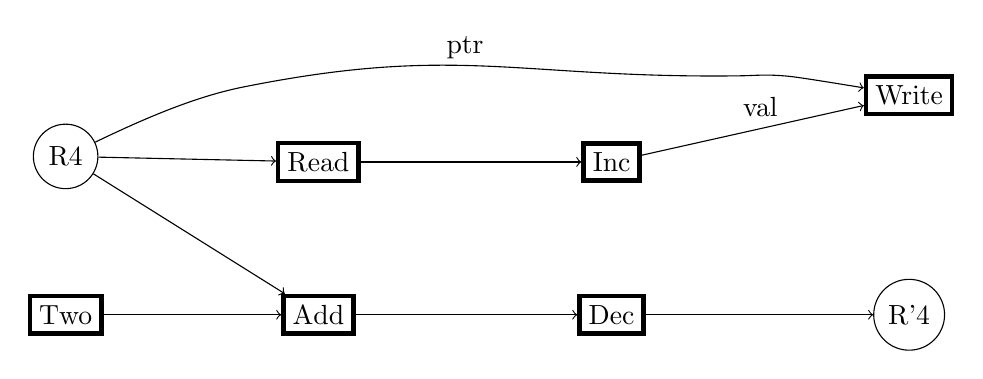
\begin{tikzpicture}[samples=100,smooth]
		%%
  \node (Read) at (118.0bp,259.0bp) [draw,rectangle,ultra thick] {Read};
  \node (Two) at (27.0bp,204.0bp) [draw,rectangle,ultra thick] {Two};
  \node (Write) at (330.66bp,283.0bp) [draw,rectangle,ultra thick] {Write};
  \node (Add) at (118.0bp,204.0bp) [draw,rectangle,ultra thick] {Add};
  \node (R4) at (27.0bp,261.0bp) [draw,circle] {R4};
  \node (R'4) at (330.66bp,204.0bp) [draw,circle] {R'4};
  \node (Dec) at (223.55bp,204.0bp) [draw,rectangle,ultra thick] {Dec};
  \node (Inc) at (223.55bp,259.0bp) [draw,rectangle,ultra thick] {Inc};
  \draw [->] (Inc) ..controls (263.64bp,267.98bp) and (279.53bp,271.54bp)  .. (Write);
  \definecolor{strokecol}{rgb}{0.0,0.0,0.0};
  \pgfsetstrokecolor{strokecol}
  \draw (277.1bp,279.0bp) node {val};
  \draw [->] (Add) ..controls (157.74bp,204.0bp) and (172.85bp,204.0bp)  .. (Dec);
  \draw [->] (R4) ..controls (55.204bp,243.33bp) and (69.205bp,234.56bp)  .. (Add);
  \draw [->] (Read) ..controls (157.74bp,259.0bp) and (172.85bp,259.0bp)  .. (Inc);
  \draw [->] (R4) ..controls (58.024bp,275.96bp) and (75.092bp,282.82bp)  .. (91.0bp,286.0bp) .. controls (168.4bp,301.48bp) and (189.62bp,289.11bp)  .. (268.55bp,290.0bp) .. controls (276.15bp,290.09bp) and (278.08bp,290.59bp)  .. (285.66bp,290.0bp) .. controls (288.21bp,289.8bp) and (290.83bp,289.54bp)  .. (Write);
  \draw (170.78bp,300.0bp) node {ptr};
  \draw [->] (Dec) ..controls (265.08bp,204.0bp) and (283.05bp,204.0bp)  .. (R'4);
  \draw [->] (Two) ..controls (62.581bp,204.0bp) and (71.822bp,204.0bp)  .. (Add);
  \draw [->] (R4) ..controls (57.446bp,260.33bp) and (69.459bp,260.07bp)  .. (Read);
		%
	\end{tikzpicture}
	\label{fig:increment-circuit}
	\caption{The circuit generated for every step by the controller, found with SHADE/current to p best/1/bin with Curriculum Learning.}
\end{figure}
\begin{table}[h]
	\centering
	\rowcolors{2}{LightGray}{white}
	\resizebox{\textwidth}{!}{\begin{tabular}{c|ccccccccccccccc|ccccc}
		\rowcolor{Gray}\textbf{Step} & 0 & 1 & 2 & 3 & 4 & 5 & 6 & 7 & 8 & 9 & 10 & 11 & 12 & 13 & 14 & \textit{r}0 & \textit{r}1 & \textit{r}2 & \textit{r}3 & \textit{r}4 \\ \hline 
1 & 12 & 12 & 12 & 10 & 1 & 12 & 10 & 1 & 10 & 1 & 13 & 14 & 4 & 11 & 0 & 0 & 0 & 13 & 0 & 1 \\ 
2 & 13 & 12 & 12 & 10 & 1 & 12 & 10 & 1 & 10 & 1 & 13 & 14 & 4 & 11 & 0 & 13 & 0 & 0 & 0 & 2 \\ 
3 & 13 & 13 & 12 & 10 & 1 & 12 & 10 & 1 & 10 & 1 & 13 & 14 & 4 & 11 & 0 & 0 & 12 & 13 & 12 & 3 \\ 
4 & 13 & 13 & 13 & 10 & 1 & 12 & 10 & 1 & 10 & 1 & 13 & 14 & 4 & 11 & 0 & 13 & 10 & 11 & 10 & 4 \\ 
5 & 13 & 13 & 13 & 11 & 1 & 12 & 10 & 1 & 10 & 1 & 13 & 14 & 4 & 11 & 0 & 11 & 1 & 2 & 1 & 5 \\ 
6 & 13 & 13 & 13 & 11 & 2 & 12 & 10 & 1 & 10 & 1 & 13 & 14 & 4 & 11 & 0 & 2 & 12 & 13 & 12 & 6 \\ 
7 & 13 & 13 & 13 & 11 & 2 & 13 & 10 & 1 & 10 & 1 & 13 & 14 & 4 & 11 & 0 & 13 & 10 & 11 & 10 & 7 \\ 
8 & 13 & 13 & 13 & 11 & 2 & 13 & 11 & 1 & 10 & 1 & 13 & 14 & 4 & 11 & 0 & 11 & 1 & 2 & 1 & 8 \\ 
9 & 13 & 13 & 13 & 11 & 2 & 13 & 11 & 2 & 10 & 1 & 13 & 14 & 4 & 11 & 0 & 2 & 10 & 11 & 10 & 9 \\ 
10 & 13 & 13 & 13 & 11 & 2 & 13 & 11 & 2 & 11 & 1 & 13 & 14 & 4 & 11 & 0 & 11 & 1 & 2 & 1 & 10 \\ 
11 & 13 & 13 & 13 & 11 & 2 & 13 & 11 & 2 & 11 & 2 & 13 & 14 & 4 & 11 & 0 & 2 & 13 & 14 & 13 & 11 \\ 
12 & 13 & 13 & 13 & 11 & 2 & 13 & 11 & 2 & 11 & 2 & 14 & 14 & 4 & 11 & 0 & 14 & 14 & 0 & 14 & 12 \\ \hline 
\rowcolor{Gray}Final & 13 & 13 & 13 & 11 & 2 & 13 & 11 & 2 & 11 & 2 & 14 & 0 & 4 & 11 & 0 & 14 & 14 & 0 & 14 & 12 \\
\end{tabular}}
	\label{tbl:increment-execution-example}
	\caption{Behaviour obtained with the task Increment.}
\end{table}
\clearpage


\clearpage
\subsection{Copy}

\begin{figure}[h]
	\centering
	\begin{tikzpicture}[>=latex',line join=bevel,samples=100,smooth, scale=.875]
		%%
		\node (R'0) at (105.0bp,22.0bp) [draw,circle] {R'0};
  		\node (R'1) at (298.1bp,193.0bp) [draw,circle] {R'1};
  		\node (R'2) at (298.1bp,40.0bp) [draw,circle] {R'2};
  		\node (R'3) at (298.1bp,102.0bp) [draw,circle] {R'3};
  		\node (R0) at (105.0bp,143.0bp) [draw,circle] {R0};
  		\node (R1) at (20.5bp,34.0bp) [draw,circle] {R1};
  		\node (Read) at (105.0bp,80.0bp) [draw,rectangle,ultra thick] {Read};
  		\node (One) at (105.0bp,200.0bp) [draw,rectangle,ultra thick] {One};
  		\node (Write) at (212.1bp,135.0bp) [draw,rectangle,ultra thick] {Write};
  		\node (Add) at (212.1bp,193.0bp) [draw,rectangle,ultra thick] {Add};
  		\node (Inc) at (212.1bp,73.0bp) [draw,rectangle,ultra thick] {Inc};
  		\draw [->] (Inc) ..controls (248.35bp,59.092bp) and (258.46bp,55.211bp)  .. (R'2);
  		\draw [->] (R0) ..controls (137.92bp,158.37bp) and (158.02bp,167.75bp)  .. (Add);
  		\draw [->] (One) ..controls (144.96bp,197.39bp) and (160.67bp,196.36bp)  .. (Add);
  		\draw [->] (Read) ..controls (144.96bp,77.388bp) and (160.67bp,76.362bp)  .. (Inc);
  		\draw [->] (R0) ..controls (139.51bp,140.42bp) and (158.18bp,139.03bp)  .. (Write);
  		\definecolor{strokecol}{rgb}{0.0,0.0,0.0};
  		\pgfsetstrokecolor{strokecol}
  		\draw (158.55bp,146.0bp) node {ptr};
  		\draw [->] (Add) ..controls (247.71bp,193.0bp) and (257.04bp,193.0bp)  .. (R'1);
  		\draw [->] (R1) ..controls (50.579bp,29.728bp) and (62.28bp,28.067bp)  .. (R'0);
  		\draw [->] (Inc) ..controls (248.28bp,85.198bp) and (258.3bp,88.578bp)  .. (R'3);
  		\draw [->] (Read) ..controls (145.35bp,100.72bp) and (161.59bp,109.06bp)  .. (Write);
  		\draw (158.55bp,117.0bp) node {val};
  		\draw [->] (R1) ..controls (47.62bp,48.764bp) and (58.462bp,54.666bp)  .. (Read);
		%
	\end{tikzpicture}
	\label{fig:copy-circuit}
	\caption{The only circuit generated by the controller, found with JADE/current to p best/1/bin.}
\end{figure}
\begin{table}[h]
	\centering
	\rowcolors{2}{LightGray}{white}
	\resizebox{\textwidth}{!}{\begin{tabular}{c|cccccccccccccccc|cccc}
		\rowcolor{Gray}\textbf{Step} & 0 & 1 & 2 & 3 & 4 & 5 & 6 & 7 & 8 & 9 & 10 & 11 & 12 & 13 & 14 & 15 & \textit{r}0 & \textit{r}1 & \textit{r}2 & \textit{r}3 \\ \hline 
1 & 8 & 11 & 15 & 5 & 8 & 13 & 8 & 3 & 0 & 0 & 0 & 0 & 0 & 0 & 0 & 0 & 0 & 0 & 0 & 0 \\ 
2 & 8 & 11 & 15 & 5 & 8 & 13 & 8 & 3 & 0 & 0 & 0 & 0 & 0 & 0 & 0 & 0 & 8 & 1 & 2 & 1 \\ 
3 & 8 & 11 & 15 & 5 & 8 & 13 & 8 & 3 & 11 & 0 & 0 & 0 & 0 & 0 & 0 & 0 & 1 & 9 & 12 & 12 \\ 
4 & 8 & 0 & 15 & 5 & 8 & 13 & 8 & 3 & 11 & 0 & 0 & 0 & 0 & 0 & 0 & 0 & 9 & 2 & 1 & 1 \\ 
5 & 8 & 0 & 15 & 5 & 8 & 13 & 8 & 3 & 11 & 15 & 0 & 0 & 0 & 0 & 0 & 0 & 2 & 10 & 0 & 0 \\ 
6 & 8 & 0 & 0 & 5 & 8 & 13 & 8 & 3 & 11 & 15 & 0 & 0 & 0 & 0 & 0 & 0 & 10 & 3 & 2 & 1 \\ 
7 & 8 & 0 & 0 & 5 & 8 & 13 & 8 & 3 & 11 & 15 & 5 & 0 & 0 & 0 & 0 & 0 & 3 & 11 & 6 & 6 \\ 
8 & 8 & 0 & 0 & 0 & 8 & 13 & 8 & 3 & 11 & 15 & 5 & 0 & 0 & 0 & 0 & 0 & 11 & 4 & 1 & 1 \\ 
9 & 8 & 0 & 0 & 0 & 8 & 13 & 8 & 3 & 11 & 15 & 5 & 8 & 0 & 0 & 0 & 0 & 4 & 12 & 9 & 9 \\ 
10 & 8 & 0 & 0 & 0 & 0 & 13 & 8 & 3 & 11 & 15 & 5 & 8 & 0 & 0 & 0 & 0 & 12 & 5 & 1 & 1 \\ 
11 & 8 & 0 & 0 & 0 & 0 & 13 & 8 & 3 & 11 & 15 & 5 & 8 & 13 & 0 & 0 & 0 & 5 & 13 & 14 & 14 \\ 
12 & 8 & 0 & 0 & 0 & 0 & 0 & 8 & 3 & 11 & 15 & 5 & 8 & 13 & 0 & 0 & 0 & 13 & 6 & 1 & 1 \\ 
13 & 8 & 0 & 0 & 0 & 0 & 0 & 8 & 3 & 11 & 15 & 5 & 8 & 13 & 8 & 0 & 0 & 6 & 14 & 9 & 9 \\ 
14 & 8 & 0 & 0 & 0 & 0 & 0 & 0 & 3 & 11 & 15 & 5 & 8 & 13 & 8 & 0 & 0 & 14 & 7 & 1 & 1 \\ 
15 & 8 & 0 & 0 & 0 & 0 & 0 & 0 & 3 & 11 & 15 & 5 & 8 & 13 & 8 & 3 & 0 & 7 & 15 & 4 & 4 \\ \hline
Final & 8 & 0 & 0 & 0 & 0 & 0 & 0 & 0 & 11 & 15 & 5 & 8 & 13 & 8 & 3 & 0 & 15 & 8 & 1 & 1 \\
	\end{tabular}}
	\label{tbl:access-execution-example}
	\caption{Behaviour obtained with the task Copy.}
\end{table}
\clearpage
\subsection{Reverse}

\begin{figure}[h]
	\centering
	\resizebox{0.4\linewidth}{!}{\begin{tikzpicture}[>=latex',line join=bevel,samples=100,smooth]
		%%
		\node (R'0) at (225.1bp,84.0bp) [draw,circle] {R'0};
        \node (R'1) at (225.1bp,236.0bp) [draw,circle] {R'1};
        \node (R'3) at (225.1bp,22.0bp) [draw,circle] {R'3};
        \node (R1) at (27.0bp,236.0bp) [draw,circle] {R1};
        \node (R3) at (27.0bp,113.0bp) [draw,circle] {R3};
        \node (Read) at (118.0bp,127.0bp) [draw,rectangle,ultra thick] {Read};
        \node (Two) at (27.0bp,179.0bp) [draw,rectangle,ultra thick] {Two};
        \node (Write) at (225.1bp,160.0bp) [draw,rectangle,ultra thick] {Write};
        \node (Inc) at (118.0bp,73.0bp) [draw,rectangle,ultra thick] {Inc};
        \node (Dec) at (118.0bp,236.0bp) [draw,rectangle,ultra thick] {Dec};
        \node (Sub) at (118.0bp,181.0bp) [draw,rectangle,ultra thick] {Sub};
        \draw [->] (Dec) ..controls (159.53bp,236.0bp) and (177.5bp,236.0bp)  .. (R'1);
        \draw [->] (R1) ..controls (55.204bp,218.95bp) and (69.205bp,210.49bp)  .. (Sub);
        \draw [->] (Sub) ..controls (158.09bp,173.14bp) and (173.97bp,170.02bp)  .. (Write);
        \definecolor{strokecol}{rgb}{0.0,0.0,0.0};
        \pgfsetstrokecolor{strokecol}
        \draw (171.55bp,179.0bp) node {ptr};
        \draw [->] (Inc) ..controls (159.63bp,77.275bp) and (177.75bp,79.137bp)  .. (R'0);
        \draw [->] (Two) ..controls (62.581bp,179.78bp) and (71.822bp,179.99bp)  .. (Sub);
        \draw [->] (R3) ..controls (56.125bp,100.2bp) and (69.19bp,94.455bp)  .. (Inc);
        \draw [->] (R1) ..controls (57.446bp,236.0bp) and (69.459bp,236.0bp)  .. (Dec);
        \draw [->] (Inc) ..controls (160.52bp,52.751bp) and (179.99bp,43.483bp)  .. (R'3);
        \draw [->] (Read) ..controls (158.09bp,139.35bp) and (173.97bp,144.25bp)  .. (Write);
        \draw (171.55bp,153.0bp) node {val};
        \draw [->] (R3) ..controls (57.446bp,117.68bp) and (69.459bp,119.53bp)  .. (Read);
		%
	\end{tikzpicture}}
	\label{fig:reverse-circuit-2}
	\caption{The circuit generated by the controller by step $\geq 2$, found with JADE/current to p best/1/bin with Curriculum Learning.}
\end{figure}
\def\arraystretch{1.0}
\begin{table}[h]
	\centering
	\rowcolors{2}{LightGray}{white}
	\resizebox{\linewidth}{!}{\begin{tabular}{c|cccccccccccc|cccc}
		\rowcolor{Gray}\textbf{Step} & 0 & 1 & 2 & 3 & 4 & 5 & 6 & 7 & 8 & 9 & 10 & 11 & \textit{r}0 & \textit{r}1 & \textit{r}2 & \textit{r}3 \\ \hline 
1 & 6 & 11 & 10 & 10 & 4 & 3 & 0 & 0 & 0 & 0 & 0 & 0 & 1 & 0 & 0 & 1 \\ 
2 & 6 & 11 & 10 & 10 & 4 & 3 & 0 & 0 & 0 & 0 & 6 & 0 & 2 & 11 & 0 & 2 \\ 
3 & 6 & 11 & 10 & 10 & 4 & 3 & 0 & 0 & 0 & 0 & 11 & 0 & 3 & 10 & 0 & 3 \\ 
4 & 6 & 11 & 10 & 10 & 4 & 3 & 0 & 0 & 0 & 10 & 11 & 0 & 4 & 9 & 0 & 4 \\ 
5 & 6 & 11 & 10 & 10 & 4 & 3 & 0 & 0 & 10 & 10 & 11 & 0 & 5 & 8 & 0 & 5 \\ 
6 & 6 & 11 & 10 & 10 & 4 & 3 & 0 & 4 & 10 & 10 & 11 & 0 & 6 & 7 & 0 & 6 \\ 
7 & 6 & 11 & 10 & 10 & 4 & 3 & 3 & 4 & 10 & 10 & 11 & 0 & 7 & 6 & 0 & 7 \\ 
8 & 6 & 11 & 10 & 10 & 4 & 3 & 3 & 4 & 10 & 10 & 11 & 0 & 8 & 5 & 0 & 8 \\ 
9 & 6 & 11 & 10 & 10 & 4 & 3 & 3 & 4 & 10 & 10 & 11 & 0 & 9 & 4 & 0 & 9 \\ 
10 & 6 & 11 & 10 & 10 & 4 & 3 & 3 & 4 & 10 & 10 & 11 & 0 & 10 & 3 & 0 & 10 \\ 
11 & 6 & 11 & 10 & 10 & 4 & 3 & 3 & 4 & 10 & 10 & 11 & 0 & 11 & 2 & 0 & 11 \\ \hline 
\rowcolor{Gray}Final & 6 & 11 & 10 & 10 & 4 & 3 & 3 & 4 & 10 & 10 & 11 & 0 & 11 & 2 & 0 & 11 \\
	\end{tabular}}
	\label{tbl:reverse-execution-example}
	\caption{Behaviour obtained with the task Reverse.}
\end{table}
\clearpage
\subsection{Swap}
TODO